\chapter{Design}

\section{System Design}

To establish common language for this thesis, following terms are defined:

\begin{itemize}
    \item sensor - the electrode pair that is submerged in the solution
    \item signal generator - the source of the AC signal
    \item signal reader - the Voltmeter measuring the voltage drop
    \item sensor node - a signal generator, reader and a number of ports to connect sensors
    \item data processing unit - a unit providing all of the above with power, controlling their functions and capturing their data to log it and make it available to a user-readable output
    \item user-interface - the interface for the user to control the system and view the data
    \item sensor system - the sum of the described subsystems
\end{itemize}

\begin{figure}
	\begin{center}
		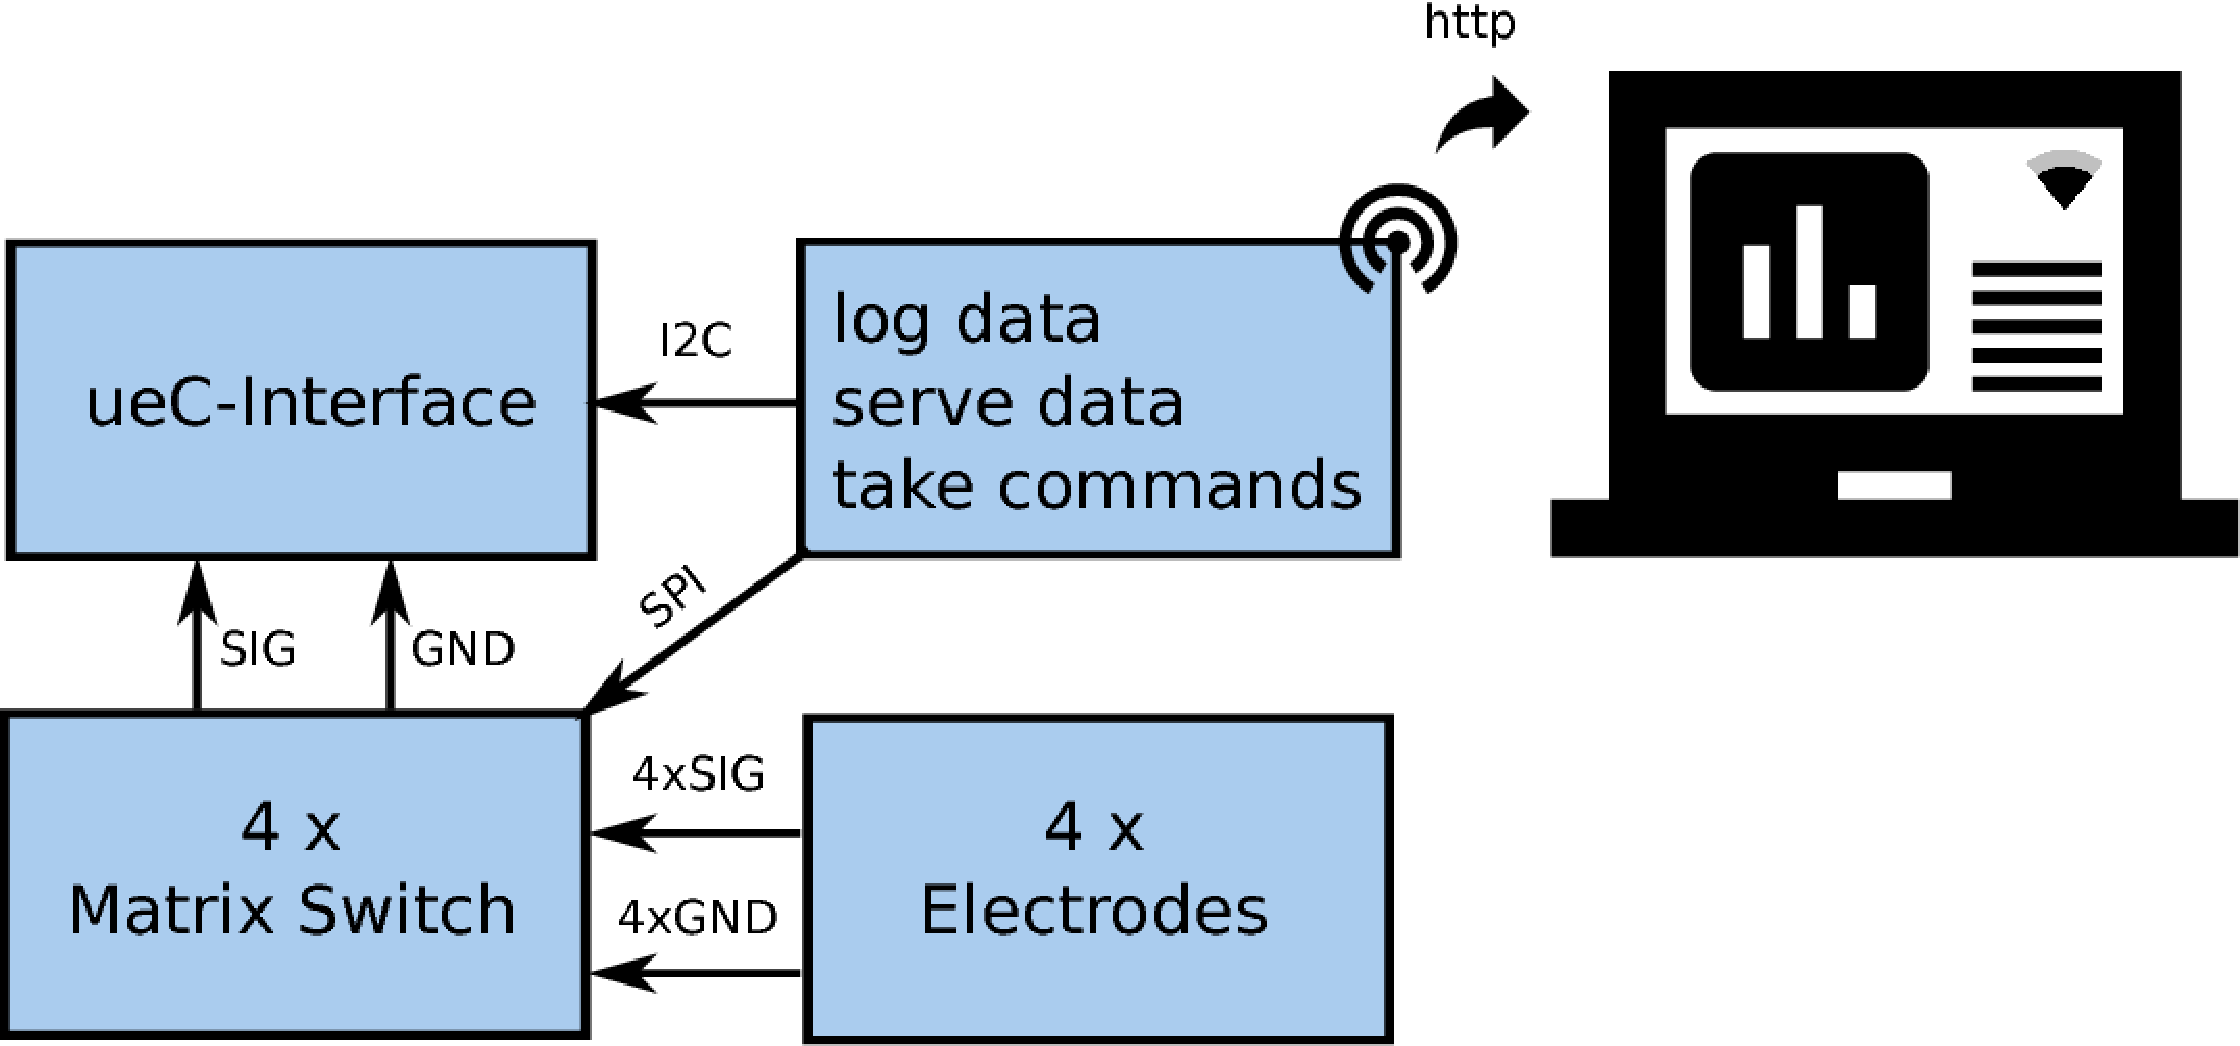
\includegraphics[width=\textwidth]{images/systemdesign.pdf} 
		\caption{System Design [why is this so ugly]}
	\end{center}
\end{figure}

\subsection{Sensors}

The sensor is a pair of electrodes submerged in the fluid. Waterproof wiring from these electrodes to the electrical interfaces is needed.

[electrode design - i.e. size, distance, form]

The first version of the sensor was made from two platinum electrodes that were wired to the sensor node via jumper cables. This was good enough to verify the function of the circuitry, but could not be deployed in the reactor in this form.

The second version of the sensor was built as a sensor array containing of multiple sensors on a sensor strip \ref{fig:v2}. A \unit[5]{cm} wide and \unit[25]{cm} long strip of Kapton adhesive tape served as the base. 4 electrode pairs made from \unit[0.2]{mm} platinum wire were arranged equidistant on the strip. \unit[0.4]{mm} enameled copper wire runs along the tape to connect each electrode pair to the left end of the strip, from which insulated cables run to the sensor node. After soldering the joints, two smaller strips of tape were used to cover the wiring, exposing only the electrodes to fluid.

First tests with this sensor array showed the viability of the concept, however a simple look at it shows the inherit problems. Instead of a uniformly flat strip with minimal influence on the flow, it provides several irregularities. Soldering \unit[0.2]{mm} platinum wire to \unit[0.4]{mm} enameled copper wire on a piece of adhesive tape per hand also did not result in clean solder joints. And while with the experience of the first array, the second array turned out a bit cleaner, the fundamental problems stay.

\begin{figure}
	\begin{center}
		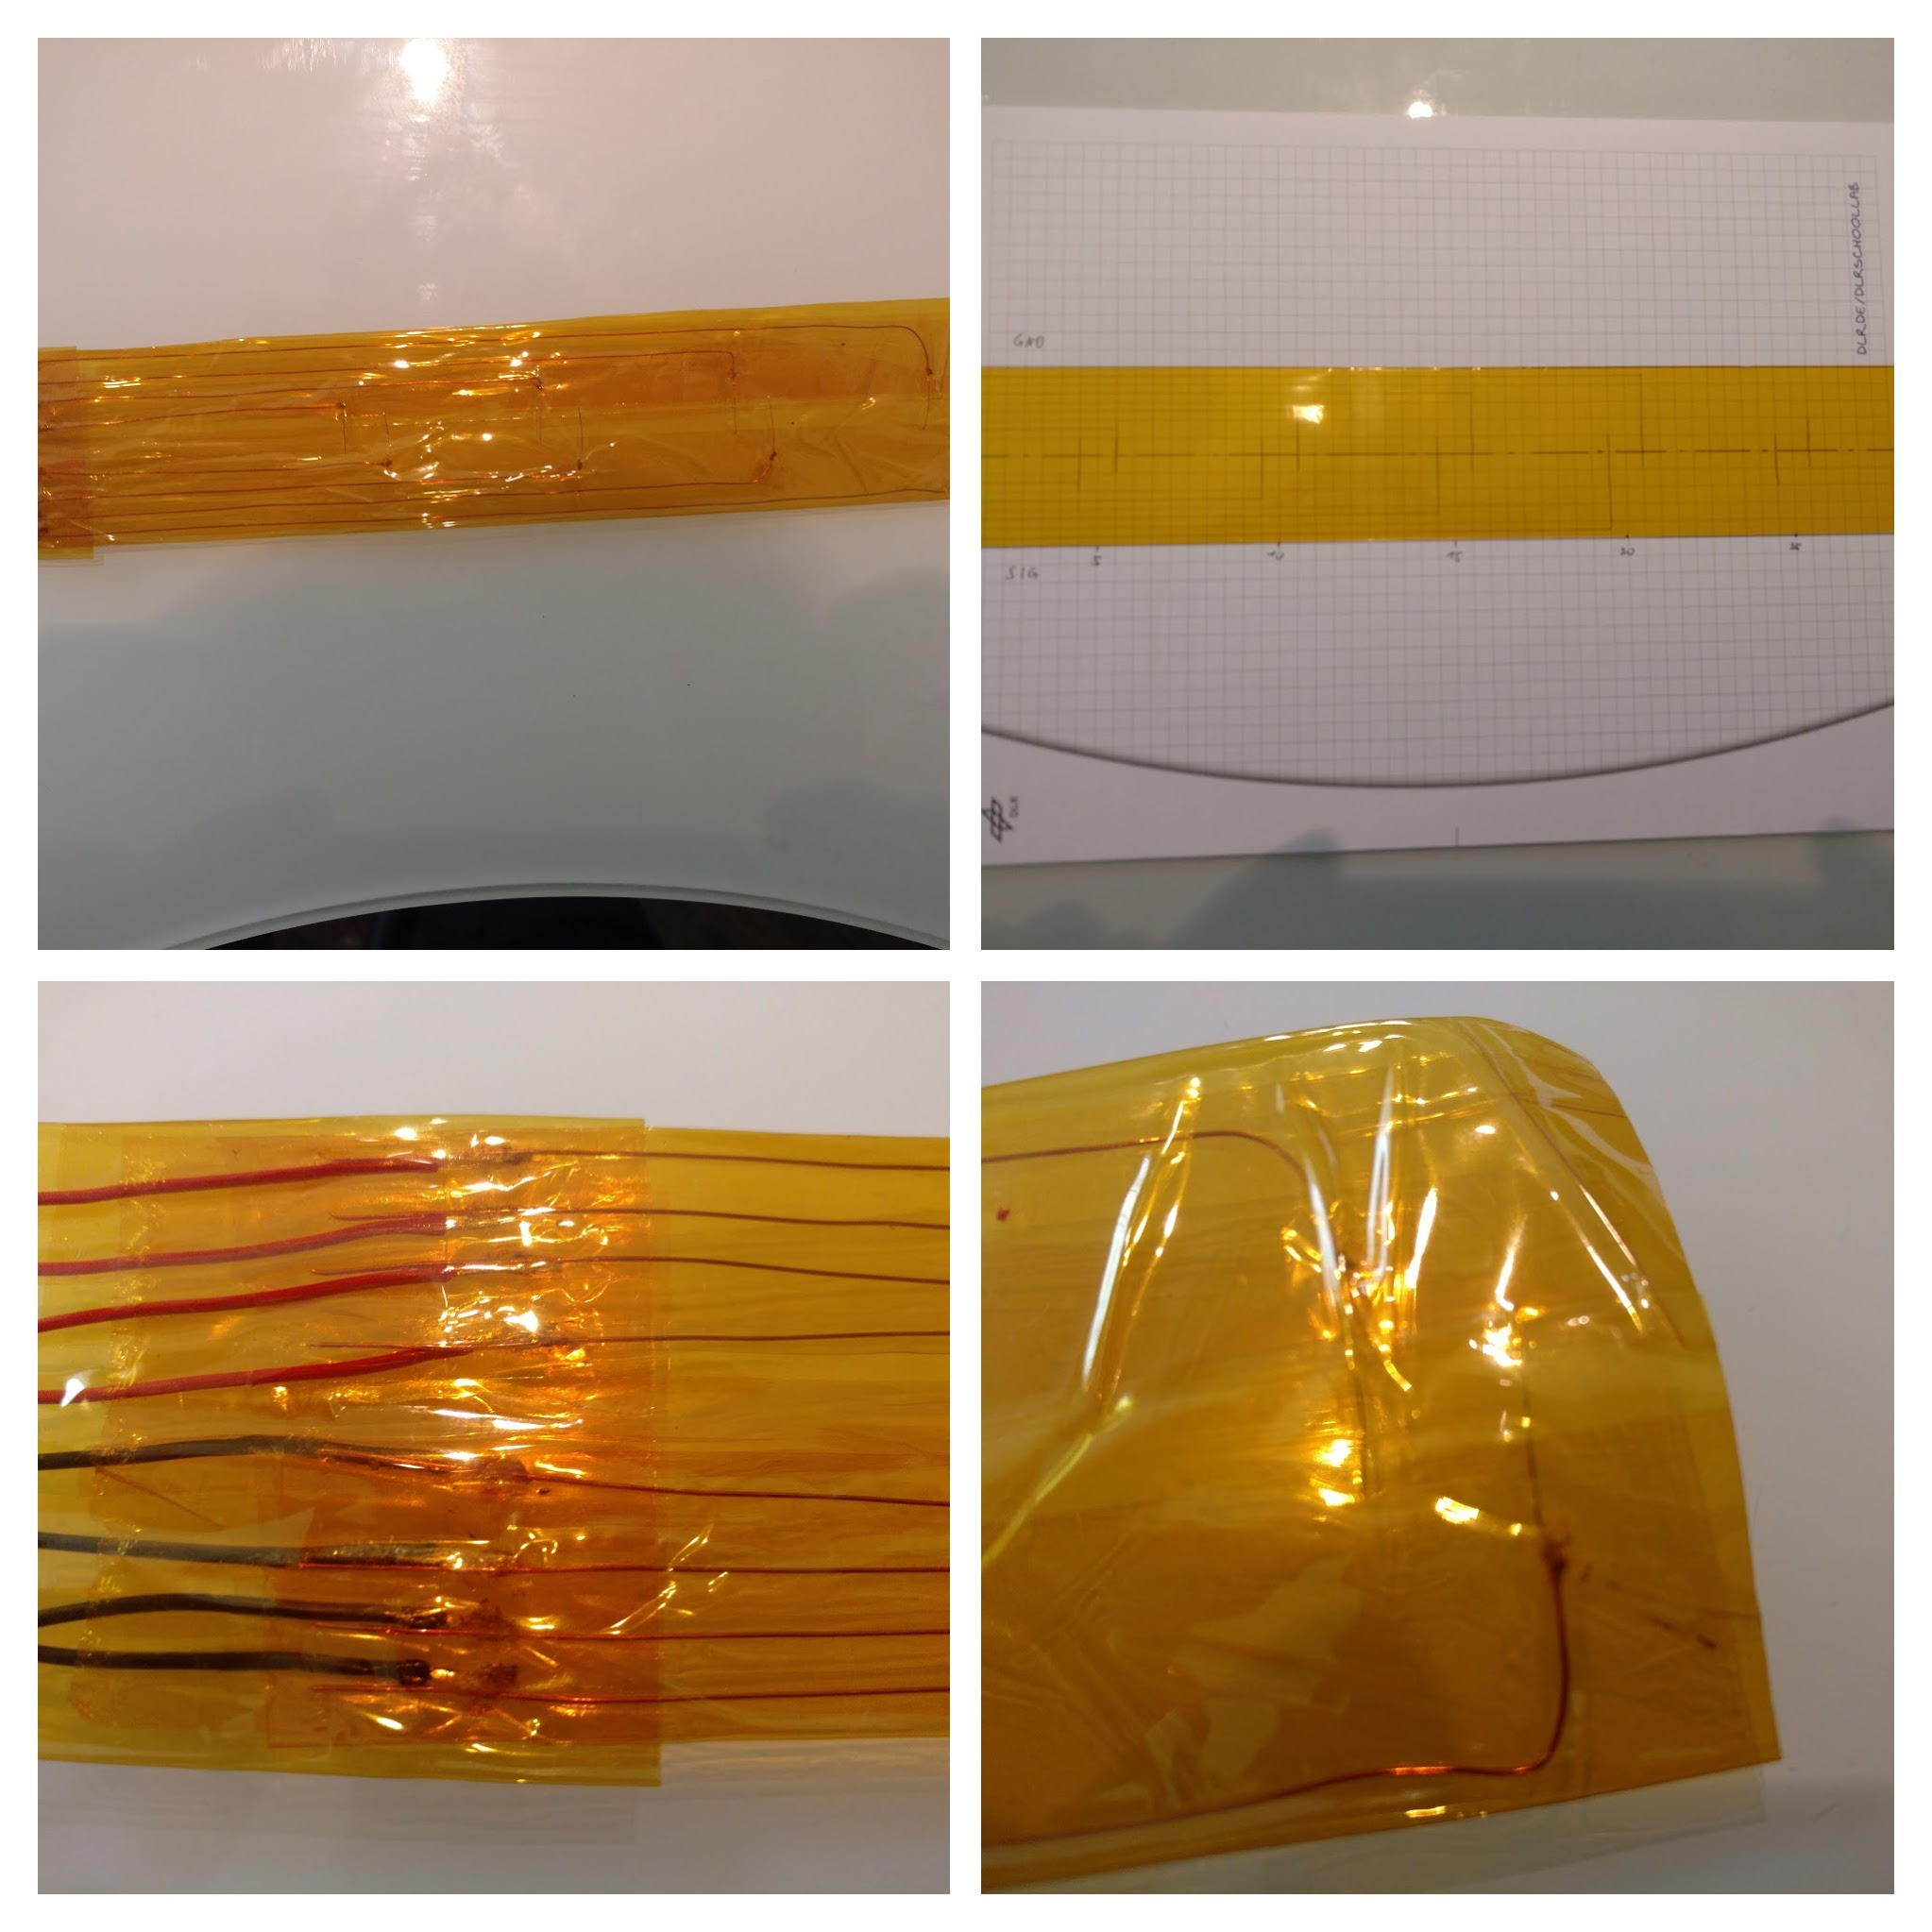
\includegraphics[width=\textwidth]{images/v2.jpg} 
		\caption{Handmade Sensor Strip}
		\label{fig:v2}
	\end{center}
\end{figure}

As an alternative to these handmade strips, industrially produced Flex-PCBs were identified. Flex-PCBs are flexible printed circuit boards that are very close to our handmade arrays. They also use Kapton as base, on which a copper coating gets applied and partially removed to form the conducting paths. On top, another layer of Kapton is applied, with cut outs in the places where the copper is supposed to be exposed. The exposed copper is then plated with ENIG (Electroless nickel immersion gold) to protect the copper from oxidation and provide the landing pads for electrical components to be solder on.
For our purpose those exposed and plated landing pads can be used as electrodes, being nicely embedded in a FlexPCB that also runs the wiring to the sensor node.

\begin{figure}
	\begin{center}
		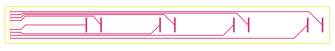
\includegraphics[width=\textwidth]{images/fpcbd.pdf} 
		\caption{Design of FlexPCB}
		\label{fig:fpcbd}
	\end{center}
\end{figure}
[image flexpcb]

[platinum vs. ENIG a electrode material]

\subsection{Sensor Node}

The sensor node logically consists of the signal generator and the signal reader, practically both parts are tightly integrated.

[Describe mini-eC-Interface]
[also where i.e. the change with the filter cap and the tests that surfaced the issue is described]

The mini-eC-Interface provides two channels to connect to the electrodes, but  multiple sensors should be driven by one interface. The method to this is called demultiplexing and the component able to this is the Matrix-Switch.
A Matrix-Switch is an electrical component containing a multitude of switches, where the switches can be electronically closed and opened from a controller. The Matrix-Switch chosen consists of 8 switches, where all switches have the same input, but separate outputs. Thus, they allow applying an input signal to different outputs. The input in our case is the signal and reference from the minie-eC-Interface, applied to 8 different electrode pairs making up the sensors. A separate Matrix-Switch is need for signal and reference.

[name of matrix switch]

This allows us to use one mini-eC-Interface to drive 8 sensors.

\subsubsection{Data Processing Unit}

The Data Processing Unit has to be able to control the functions of the sensor nodes attached to it, read the data from them, log it and serve it to the user-interface. Typically, any micro-controller is is fit for those tasks. Micro-controllers usually are programmed in C or C++, however nowadays there are other options, too. One of those is Micropython, which is an implementation of the Python 3 programming language designed to run on micro-controllers. Python is a vastly easier language than C/C++, and this is especially true when the involved persons are not from a computer science or electrical engineering background, but i.e. mechanical engineering or other sciences. In those fields, Python is often familiar from usage for data processing and visualization. Using Micropython enables us to design a system where it is more likely that the people using it are able to understand the code, enabling them to improve it and adapt it to alternate use-cases.
It does however limit our choice of Hardware to supported platforms and it requires more powerful and thereby expensive micro-controllers. But as the system only requires one Data Processing unit to drive a very large amount of sensors, the added cost is relative and outweighed by the benefits of the better usability. While the factor of the expensive controllers to cheaper ones is about 10, the cost in the end is still only about \euro{7}.
For prototyping, a development board named "Espruino Pico" was chosen. It is a very small and simple board that provides the electrical boilerplate to use a micro-controller without needing to deal with the lowest level of electronics, like cleaning power supply, etc.

\subsection{User-Interface}

\subsection{Sensor System}

[pcb, assembly]
